%-----------------------------------------------------------------------
%
%   UFRJ  - Universidade Federal do Rio de Janeiro
%   COPPE - Coordenação dos Programas de Pós-graduação em Engenharia
%   PEE   - Programa de Engenharia Elétrica
%
%
%   Projeto EMMA - 
%
%                                                        10/jul/15, Rio
%                                                        Ramon R. Costa
%----------------------------------------------------------------------
%
%  Compilar usando PDFLaTeX
%
%----------------------------------------------------------------------
\documentclass[12pt,a4paper]{article}
\usepackage{macros/ROSApackages} 

%-----------------------------------------------------------------------
%
%   UFRJ  - Universidade Federal do Rio de Janeiro
%   COPPE - Coordena��o dos Programas de P�s-gradua��o em Engenharia
%   PEE   - Programa de Engenharia El�trica
%
%
%   Projeto ROSA - Rob� para opera��o de stoplogs alagados
%
%   Settings
%                                                         Ramon R. Costa
%                                                         20/mar/14, Rio
%-----------------------------------------------------------------------

%---------------------------------------------------------- COLORS -----
%--------------------------------------------------- Bright colors -----
\definecolor{brightred}     {rgb}{1.00, 0.95, 0.95}
\definecolor{brightgreen}   {rgb}{0.95, 1.00, 0.95}
\definecolor{brightblue}    {rgb}{0.95, 0.95, 1.00}

\definecolor{brightyellow}  {rgb}{1.00, 1.00, 0.95}
\definecolor{brightmagenta} {rgb}{1.00, 0.95, 1.00}
\definecolor{brightcyan}    {rgb}{0.95, 1.00, 1.00}

\definecolor{brightorange}  {rgb}{1.00, 0.95, 0.85}

%----------------------------------------------------- Pale colors -----
\definecolor{palered}     {rgb}{1.00, 0.85, 0.85}
\definecolor{palegreen}   {rgb}{0.85, 1.00, 0.85}
\definecolor{paleblue}    {rgb}{0.85, 0.85, 1.00}

\definecolor{paleyellow}  {rgb}{1.00, 1.00, 0.85}
\definecolor{palemagenta} {rgb}{1.00, 0.85, 1.00}
\definecolor{palecyan}    {rgb}{0.85, 1.00, 1.00}

\definecolor{paleorange}  {rgb}{1.00, 0.85, 0.65}

%---------------------------------------------------- Light colors -----
\definecolor{lightred}     {rgb}{0.95, 0.00, 0.00}
\definecolor{lightgreen}   {rgb}{0.00, 0.95, 0.00}
\definecolor{lightblue}    {rgb}{0.00, 0.00, 0.95}

\definecolor{lightyellow}  {rgb}{0.95, 0.95, 0.00}
\definecolor{lightmagenta} {rgb}{0.95, 0.00, 0.95}
\definecolor{lightcyan}    {rgb}{0.00, 0.95, 0.95}

\definecolor{lightgray}    {rgb}{0.95, 0.95, 0.95}

\definecolor{lightorange}  {rgb}{0.95, 0.63, 0.00}

%--------------------------------------------------- Middle colors -----
\definecolor{midred}     {rgb}{0.85, 0.00, 0.00}
\definecolor{midgreen}   {rgb}{0.00, 0.85, 0.00}
\definecolor{midblue}    {rgb}{0.00, 0.00, 0.85}

\definecolor{midyellow}  {rgb}{0.85, 0.85, 0.00}
\definecolor{midmagenta} {rgb}{0.85, 0.00, 0.85}
\definecolor{midcyan}    {rgb}{0.00, 0.85, 0.85}

\definecolor{midgray}    {rgb}{0.85, 0.85, 0.85}

\definecolor{midorange}  {rgb}{0.85, 0.57, 0.00}

%--------------------------------------------------- Normal colors -----
\definecolor{red}     {rgb}{0.75, 0.00, 0.00}
\definecolor{green}   {rgb}{0.00, 0.75, 0.00}
\definecolor{blue}    {rgb}{0.00, 0.00, 0.75}

\definecolor{yellow}  {rgb}{0.75, 0.75, 0.00}
\definecolor{magenta} {rgb}{0.75, 0.00, 0.75}
\definecolor{cyan}    {rgb}{0.00, 0.75, 0.75}

\definecolor{gray}    {rgb}{0.75, 0.75, 0.75}

\definecolor{orange}  {rgb}{0.75, 0.50, 0.00}

%--------------------------------------------------- Shadow colors -----
\definecolor{shadred}     {rgb}{0.65, 0.00, 0.00}
\definecolor{shadgreen}   {rgb}{0.00, 0.65, 0.00}
\definecolor{shadblue}    {rgb}{0.00, 0.00, 0.65}

\definecolor{shadyellow}  {rgb}{0.65, 0.65, 0.00}
\definecolor{shadmagenta} {rgb}{0.65, 0.00, 0.65}
\definecolor{shadcyan}    {rgb}{0.00, 0.65, 0.65}

\definecolor{shadgray}    {rgb}{0.65, 0.65, 0.65}

\definecolor{shadorange}  {rgb}{0.65, 0.43, 0.00}

%--------------------------------------------------- Darker colors -----
\definecolor{darkred}     {rgb}{0.50, 0.00, 0.00}
\definecolor{darkgreen}   {rgb}{0.00, 0.50, 0.00}
\definecolor{darkblue}    {rgb}{0.00, 0.00, 0.50}

\definecolor{darkyellow}  {rgb}{0.50, 0.50, 0.00}
\definecolor{darkmagenta} {rgb}{0.50, 0.00, 0.50}
\definecolor{darkcyan}    {rgb}{0.00, 0.50, 0.50}

\definecolor{darkgray}    {rgb}{0.50, 0.50, 0.50}

\definecolor{darkorange}  {rgb}{0.50, 0.33, 0.00}

%-------------------------------------------------- Hyperref setup -----
\hypersetup{
  breaklinks   = true,
  colorlinks   = true,
  linkcolor    = darkblue,
  anchorcolor  = darkcyan,
  citecolor    = darkred,
  filecolor    = darkorange,
  menucolor    = darkmagenta,
  urlcolor     = darkgreen,
  pdfhighlight = /I,
  pdfstartview = FitH,
  pdfview      = FitH
}

%---------------------------------------------- DOCUMENT STRUCTURE -----

%------------------------------------------------- Page appearance -----
\setlength{\textheight    }{250mm}
\setlength{\textwidth     }{175mm}
\setlength{\footskip      }{10mm}
\setlength{\footnotesep   }{5mm}
\setlength{\headheight    }{10mm}
\setlength{\headsep       }{5mm}
\setlength{\oddsidemargin }{-6mm}
\setlength{\evensidemargin}{-6mm}
\setlength{\topmargin     }{-15.4mm}
\setlength{\marginparsep  }{0pt}
\setlength{\marginparwidth}{0pt}
\setlength{\parindent     }{5mm}
\setlength{\parskip       }{2.5mm}
\setlength{\topmargin     }{-14mm}
\setlength{\columnsep     }{6mm}

\newcommand{\setbaselinestretch}[1]{\renewcommand{\baselinestretch}{#1}}

\newcommand{\setpagecounter}[1]{\setcounter{page}{#1}}

\setbaselinestretch{1.2}

%------------------------------------------------------- Numbering -----
\setcounter{secnumdepth}{3}  % Subsubsection numbering.
\setcounter{tocdepth}{3}     % Subsubsection index.


%---x---

%-----------------------------------------------------------------------
%
%   UFRJ  - Universidade Federal do Rio de Janeiro
%   COPPE - Coordena��o dos Programas de P�s-gradua��o em Engenharia
%   PEE   - Programa de Engenharia El�trica
%
%
%   Projeto ROSA - Rob� para opera��o de stoplogs alagados
%
%   Macros
%                                                         Ramon R. Costa
%                                                         20/mar/14, Rio
%-----------------------------------------------------------------------

%-------------------------------------------------- Text highlight -----
\newcommand{\texthfg}[1]{\textcolor{blue}{#1}}
\newcommand{\texthbg}[1]{\fcolorbox{lightgray}{lightgray}{#1}}
\newcommand{\HI}[1]{\colorbox{yellow}{\textcolor{black}{#1}}}  %% Highlithed text

\newcommand{\BLU}[1]{\colorbox{white}{\textcolor{blue}{#1}}}

%--------------------------------------------------------- Bullets -----
\renewcommand{\labelitemi}{\texthfg{$\bullet$}}                          % First level.
\renewcommand{\labelitemii}{\texthfg{\tiny$\blacksquare$}}               % Second level.
\renewcommand{\labelitemiii}{\texthfg{\scriptsize$\blacktriangleright$}} % Third level.
\renewcommand{\labelitemiv}{\texthfg{\scriptsize$\bigstar$}}             % Fourth level.

%----------------------------------------------------- Date & time -----
\newcount\m
\newcount\n

\def\twodigits#1{\ifnum #1<10 0\fi \number#1}

\def\hours{\n=\time \divide\n 60
  \m=-\n \multiply\m 60 \advance\m \time
  \twodigits\n:\twodigits\m}

\def\hora{\hours}

\def\data{Rio de Janeiro,\  \number\day\  de \ifcase\month\or
  janeiro\or
  fevereiro\or
  mar\c{c}o\or
  abril\or
  maio\or
  junho\or
  julho\or
  agosto\or
  setembro\or
  outubro\or
  novembro\or
  dezembro\or\fi\  de \number\year
}

%---------------------------------------------------------- Useful -----
\def\pee{Programa de Engenharia El�trica\xspace}
\def\PEE{PROGRAMA DE ENGENHARIA EL�TRICA\xspace}

\def\coppe{Coordena��o dos Programas de P�s--Gradua��o em Engenharia\xspace}
\def\COPPE{COORDENA��O DOS PROGRAMAS DE P�S--GRADUA��O EM ENGENHARIA\xspace}

\def\ct{Centro de Tecnologia\xspace}
\def\CT{CENTRO DE TECNOLOGIA\xspace}

\def\ufrj{Universidade Federal do Rio de Janeiro\xspace}
\def\UFRJ{UNIVERSIDADE FEDERAL DO RIO DE JANEIRO\xspace}

\def\rrc{Ramon Romankevicius Costa\xspace}
\def\RRC{RAMON ROMANKEVICIUS COSTA\xspace}

\def\gscar{Gru\-po de Si\-mu\-la\-��o e Con\-tro\-le em Auto\-ma\-��o e Ro\-b�\-ti\-ca\xspace}
\def\GSCAR{GRUPO DE SIMULA��O E CONTROLE EM AUTOMA��O e ROB�TICA\xspace}

%------------------------------------------------------------ ROSA -----
\def\ROSA{\texthfg{ROSA}}
\def\LROSA{\ROSA\ -- \textit{Stoplog Inspection}}

%\def\ROSA{\BLU{\textsc{ROSA}}\xspace}

%----------------------------------------------------------------------
\newfont{\grande}{cmss10 scaled 1500}
\newfont{\Grande}{cmss10 scaled 2500}
\newfont{\GRANDE}{cmss10 scaled 3500}
\newfont{\enorme}{cmdunh10 scaled 6000}

\newcommand{\block}[2]{
  \def\TXT{~#1~}
  \noindent\TXT \hfill
  \parbox[t]{ \textwidth - \widthof{\TXT} - 2mm}{#2} \\
}

\newcommand{\participantes}[1]{
  \block{\textbf{Participantes}:}{#1}
  \medskip%
}

\newcommand{\pauta}[1]{
  \block{\textbf{Pauta}:}{#1}
  \medskip%
}

\newcommand{\dado}[2]{
  \noindent%
  \makebox[30mm][l]{\sf#1 {\small\dotfill}} :
  \hfill\parbox[t]{140mm}{#2} %\\[2mm]
  \par
  \vspace*{0.30mm}
}

\newcommand{\vu}[2]{ %Utiliza��o: \vu{valor}{unidade}
  \textcolor{darkblue}{#1$\,#2$}\xspace
}

\def\alana{Alana Monteiro\xspace}
\def\antonio{Ant�nio\xspace}
\def\jacoud{Alessandro Jacoud\xspace}
\def\andre{Andr� Figueir�\xspace}
\def\breno{Breno Bellinati de Carvalho\xspace}
\def\elael{Eduardo Elael\xspace}
\def\gabriel{Gabriel Alc�ntara\xspace}
\def\gizele{Gizele Ferreira da Silva\xspace}
\def\julia{J�lia Campana\xspace}
\def\patrick{Patrick Paranhos\xspace}
\def\rafael{Rafael Oliveira\xspace}
\def\ramonC{Ramon Campos\xspace}
\def\ramon{Ramon Romankevicius\xspace}
\def\renan{Renan Freitas\xspace}
\def\sylvain{Sylvain Joyeux\xspace}

\newcommand{\coordenador}{
  \vspace{1.5cm}
  \hspace{7cm}
  \parbox{7cm}{
    \centering
    \rule[0mm]{70mm}{0.1mm} \\
    \rrc \\[3mm]
    Coordenador do Projeto \\
  }
}

\def\assinaturadocoordenador{
  \vspace{10mm}%
  \parbox[t]{70mm}{
    Aprovado por: \\[5mm]
    \centering
    \includegraphics[width=65mm]{../assinatura/assinatura-digital.jpg} \\[-4mm]
    \rule[2mm]{70mm}{0.1mm} \\
    \rrc \\[3mm]
    Coordenador do Projeto \\
  }
}

\newcommand{\footnotecomendereco}{
  \vfill
  \noindent\rule[0mm]{\textwidth}{0.1mm}
  {\scriptsize \sf
  \begin{minipage}{1.5cm}
    Endere�o :
  \end{minipage}
  \begin{minipage}[t]{8.5cm}
    \rrc \\
    COPPE/UFRJ --- \pee \\
    Caixa Postal 68504 --- CEP 21941-972 \\
    Rio de Janeiro, RJ, Brasil
  \end{minipage}
  \hfill
  \begin{minipage}[t]{4cm}
    \begin{tabbing}
      e-mail\ \= : {\tt ramon@coep.ufrj.br} \\
      Lab.    \> : (21) 3938-8604 \\
      Cel.    \> : (21) 98887-9355
    \end{tabbing}
  \end{minipage}
  }
}

\newcommand{\remetente}{
  \vspace{3cm}
  \parbox{15cm}{
    \rrc \\
    COPPE/UFRJ --- \pee \\
    Caixa Postal 68.504 --- CEP 21941-972 \\
    Rio de Janeiro, RJ
  }
}

\newcommand{\fim}{
  \medskip
  \begin{center}
  \rule[1mm]{30mm}{0.14mm}$\diamond$\rule[1mm]{30mm}{0.14mm}
  \end{center}
}

%---x---

%\def\PATH{file:c:/Users/Ramon/My Documents/projetos/2015/Projeto EMMA}

\begin{document}
%---------------------------------------------------------------------
%-----------------------------------------------------------------------
%
%   UFRJ  - Universidade Federal do Rio de Janeiro
%   COPPE - Coordenação dos Programas de Pós-graduação em Engenharia
%   PEE   - Programa de Engenharia Elétrica
%
%
%   Projeto EMMA - Metodologia para revestimento robótico de turbinas in situ
%
%                                                        10/jul/15, Rio
%                                                        Ramon R. Costa
%----------------------------------------------------------------------
\pagestyle{fancy}%
\thispagestyle{fancy}%
\renewcommand{\headrulewidth}  {0.4pt}%
\renewcommand{\footrulewidth}  {0.4pt}%
\lhead{\vspace*{-5mm}
\includegraphics[width=30mm]{logo/lead-logo.jpg}}%
\chead{}%
\rhead{}%
\lfoot{}%
\cfoot{}%
\rfoot{\sf [\hours] \quad \today}%
%---------------------------------------------------------------------
\vspace*{20mm}%

{\grande \textcolor{gray}{Financiamento}}

\vspace{-25mm}%
\hspace{50mm}%

\includegraphics[width=50mm]{logo/esbr-logo.png}
\hspace{10mm}%

\includegraphics[width=40mm]{logo/aneel-logo.jpg}

\vspace{35mm}%
{\grande \textcolor{gray}{Execução}}

\vspace{-25mm}%
\hspace{50mm}%

\includegraphics[width=50mm]{logo/gscar-logo.png}
\hspace{10mm}%
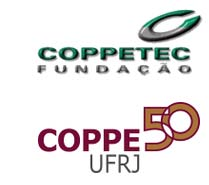
\includegraphics[width=40mm]{logo/coppetec50-logo.jpg}

\vfill%
\begin{center}
  {\GRANDE \raisebox{1.4ex}{} 
\includegraphics[width=80mm]{logo/projeto-EMMA-logo.jpg}} \\[10mm]
  %{\GRANDE \raisebox{1.4ex}{Projeto EMMA} } \\[10mm]
  {\Grande Metodologia para revestimento robótico de turbinas in situ} \\[25mm]
  {\Grande Relatório de viagem} \\[20mm]
  {\large CITENEL, Costa do Sauípe, BA} \\[5mm]
  {\large 16 a 19 de Agosto de 2015}
  \vfill%
  %{\Large \today} \\[8mm]
\end{center}

\newpage%
%---------------------------------------------------------------------
\pagestyle{fancy}%
\thispagestyle{fancy}%
\renewcommand{\headrulewidth}  {0.4pt}%
\renewcommand{\footrulewidth}  {0.4pt}%
\lhead{\vspace*{-6mm}
\includegraphics[width=30mm]{logo/lead-logo.jpg}}%
\chead{\vspace*{-6mm}\raisebox{1.7ex}{} 
\includegraphics[width=25mm]{logo/projeto-EMMA-logo.jpg}}%
%\chead{\vspace*{-6mm}\raisebox{1.7ex}{Projeto EMMA}}%
\rhead{\sf\thepage}%
\lfoot{Relatório de viagem}%
\cfoot{}%
\rfoot{\sf [\hours] \quad \today}%
%---------------------------------------------------------------------

%---------------------------------------------------------------------
%\tableofcontents

\newpage%
%---------------------------------------------------------------------
\section{Identificação}

%-----------------------------------------------------------------------
%
%   UFRJ  - Universidade Federal do Rio de Janeiro
%   COPPE - Coordenação dos Programas de Pós-graduação em Engenharia
%   PEE   - Programa de Engenharia Elétrica
%
%
%   Projeto EMMA - Metodologia para revestimento robótico de turbinas in situ
%
%   Identificação
%                                                         Ramon R. Costa
%                                                         07/jul/15, Rio
%-----------------------------------------------------------------------
%\section{Identificação}

\dado{Título}{
  EMMA - Metodologia para revestimento robótico de turbinas \textit{in situ} \\
}

\dado{Proponente}{
  Universidade Federal do Rio de Janeiro (UFRJ) \\[2mm]
  Fundação Coordenação de Projetos, Pesquisas e Estudos Tecnológicos (COPPETEC) \\
}

\dado{Contratante}{
  ESBR - Energia Sustentável do Brasil S.A. \\
}

\dado{Execução}{
  Grupo de Simulação e Controle em Automação e Robótica (GSCAR) \\
}

 \dado{Contrato}{
   Jirau 09-15 \\
 }

 \dado{P\&D ANEEL}{
   6631-0003/2015 \\
 }

%\dado{COPPETEC}{
%  N.D. \\
%}

\dado{Início}{
  26/02/2015 \\
}

\dado{Prazo}{
  14 meses \\
}

\dado{Orçamento}{
  R\$ 2.487.473,47 \\
}

\dado{Coordenador}{
  Ramon Romankevicius Costa \\
}

\dado{Gerente}{
  Breno Bellinati de Carvalho \\
}

Os engenheiros Renan Salles de Freitas e Eduardo Elael de Melo Soares
participaram do congresso e são responsáveis pela elaboração deste relatório
técnico.

%---------------------------------------------------------------------
\fim

\newpage%
%---------------------------------------------------------------------
\section{Sobre a visita}
Foram quatro dias de viagem à Costa do Sauípe, onde foi realizado o congresso
CITENEL e SEENEL:

Dia 16/08/2015:
\begin{itemize}
  \item Viagem e acomodação;
  \item Credenciamento no evento e planejamento de palestras técnicas;
\end{itemize}

Dia 17/08/2015:
\begin{itemize}
  \item Cerimônia de abertura e lançamento de revistas P\&D e EE da ANEEL;
  \item Palestra Magna - Prof. José Sidnei Colombo;
  \item Sessões técnicas;
\end{itemize}

Dia 18/08/2015:
\begin{itemize}
  \item Sessões técnicas;
\end{itemize}

Dia 19/08/2015:
\begin{itemize}
  \item Sessões técnicas;
  \item Viagem de volta;
\end{itemize}

%---------------------------------------------------------------------
\section{Considerações gerais}
A Agência Nacional de Enerngia Elétrica (ANEEL) entregou ao público a oitava
edição do Congresso de Inovação Tecnológica em Energia Elétrica (CITENEL) e a
quarta edição do Seminário de Eficiência Energética no Setor Elétrico (SEENEL),
realizados na Costa do Sauípe, Bahia, durante os dias 17, 18 e 19 de Agosto de
2015. O objetivo é ampliar a divulgação dos resultados alcançados nos
programas de Pesquisa e Desenvolvimento (P\&D) e de Eficiência Energética (EE)
regulados pela ANEEL.

A cerimônia de abertura e a palestra Magna abordaram os temas de inovação e
eficiência para o setor elétrico brasileiro, a importância da prática de
sustentabilidade, a preocupação com segurança do trabalho e primeiros socorros.

As sessões técnicas abordaram os seguintes temas: 1) redes inteligentes; 2)
planejamento de sistemas de energia elétrica; 3) geração termelétrica; 4)
eficiência energética; 5) fontes alternativas de geração de energia elétrica; 6)
supervisão, controle e proteção de sistemas de energia elétrica; 7) novos
materiais; 8) baixa renda; 9) qualidade e confiabilidade dos serviçõs de energia
elétrica; 10) medição, faturamento e combate a perdas comerciais; 11) operação
de sistemas de energia elétrica; 12) meio ambiente; 13) fontes alternativas de
geração de energia elétrica; comércio e serviços/industrial/fontes incentivadas
de energia elétrica; 14) educacional / residencial / iluminação pública; 15)
poder público; 16) segurança; 17) serviço público.

As sessões técnicas ocorriam concomitantemente, portanto foi elaborada uma
metodologia para selecionar as palestras de maior interesse para o grupo. 

\section{Planejamento de sessões técnicas}
O planejamento de sessões técnicas é a metodologia criada para a seleção das
vinte palestras técnicas com maior interesse para o grupo. Como o congresso
forneceu, durante o credenciamento, todos os artigos que seriam apresentados,
foi possível selecioná-los pelo conteúdo e resultados. O grupo selecionou os
artigos que se distinguiram pela inovação tecnológica relacionados à robótica,
sensores, e sistemas que integram hardware e software no estado da arte.

Cada sessão possui 15 minutos de apresentação e 5 minutos para perguntas.

\section{Sessões técnicas}
Nesta seção, são apresentadas as principais características e aspectos técnicos
que o grupo identificou em cada sessão. As seguintes sessões técnicas foram
presenciadas:

\textbf{Desenvolvimento de veículo dubaquático para inspeção de usinas
hidrelétricas:}
Desenvolvimento de um ROV de dimensões 400x400x600 mm de fibra de vidro com
câmeras e SONAR, e um sistema de navegação com algoritmo de Monte
Carlo e validação com câmera de alta precisão. O robô assemelha-se muito ao ROV
da empresa Seabotix em sua composição mecânica, designer, sensores e distribuição de atuadores. Como o investimento
não foi alto, os atuadores não são comerciais, mas sim projetados em Solidworks
(mecânica) e Proteus (eletrônica), e montados pela própria USP, sendo capaz de
suportar correntezas de 2 m/s. O robô foi testado em usinas
hidrelétricas e foram observado ruídos eletromagnéticos na transmissão de
imagens, sendo este o desafio para a continuação do projeto.
 %Renan

\textbf{Robô de Inspeção de Linha -D311 :}

O palestrante apresentou o desenvolimento de um robô biomimético para inspeção
em linhas de transmissão de até 138kV. Possui sua estrutura inspirada em uma
lagarta de forma a ser capaz de atravessar obstáculos que apareçam.

O projeto foi feito com sua interface em ROS que é um framework livre. O
palestrante também ressaltou que o robô possuia avanços com relação a sua versão
anterior, como uma redução de 9kg pelo uso de titânio aeronáutico e formas ovais
para os elos, que minimizaram o ruído eletromagnético. 

Durante a sessão de perguntas o palestrante concluiu, explicando que a autonomia
do robô deverá ser expantida pelo uso de indução magnética, colhendo a energia
que passa pelo fio. Atualmente ele foi desenvolvido para ser introduzido nos
pontos de ancoragem de linha, porém o projeto para um robô de resgate já
foi desenvolvido pelo mesmo laboratório.
 %Elael
\textbf{Estratégias para redução da temepratura de operação de módulos
fotovoltaicos:}
Estudo de tecnologias de redução da temperatura em módulos fotovoltaicos. Foram
estudados sistemas ativos, como ventilação forçada, e sistemas passivos,  como
aletas (material de alumínio mais comum para resfriamento)
 %Renan
%
\textbf{Desenvolvimento de Novos Coletores Solares de Condicionamento de Ar e
Refrigeração :}

O mercado crescente de ar condicionado propiciou um ambiente favoravel para o
aprimoramento de sistemas de condicionamento solares. A tecnologia de ar
condicionado solar foi dividido em duas, os de absorção e adsorção. Além deles,
existem os sistemas solares dessecantes que desumidificam o ar, atuando, assim,
 pelo uso do calor latente da água.
 O desenvolvimento do ar condicionado solar exposto na paletra foi pautado em
 simulações de volumes finitos feitos no software Ansys CFX, com criação de
 malhas através dos métodos \textit{sweep}, \textit{thin sweep} e
 \textit{inflation}. O sistema atingiu 74\% de eficiência na simulação, ficando
 ligeiramente abaixo no protótipo real.

\textbf{Sistema eletrônico de captação e direcionamento de iluminação natural
para edificações utilizando fibras ópticas - girassol eletrônico:}
A motivação para a pesquisa é a baixa eficiência (5\%) de painéis FV e a
utilização da luz natural como luz para a estação de trabalho (escritório). O
sistema tem um mecanismo que rastreia o sol com um sistema Pan e Tilt e três
sensores de luz. A fibra óptica transmite a luz solar até o ambiente de trabalho
e promete eficiência de 20 a 30\%. Foram encontrados problemas em relação ao
aquecimento da fibra e duas soluções foram abordadas: solução óptica com filtros
UV e IR; e dissipador por um sistema de refrigeração com água. O último
mostrou-se mais eficiente, porém o rendimento atual observado é 5.92\% para 5 m
de fibra óptica.
 %Renan

\textbf{Sistema de Reaproveitamento de Calor para Utilização em Banhos,
Funcionamento, Resultados e Comprovação Pro Medição e Verficação :}
 %Elael

\textbf{Equipamento com reconhecimento dinâmico de imagem para avaliação de
medidores de energia elétrica em campo:}

Apresentação de um equipamento medidor de consumo de energia elétrica, cujo
desenvolvimento teve duas motivações principais: verificar irregularidades na
rede elétrica, como erro de medição e precisão do medidor, e furto de rede
elétrica, conhecido popularmente como ``gato''. A principal característica do
dispositivo é sua facilidade de instalação, que pode ser realizada mesmo
com o medidor em funcionamento. São necessárias medidas de tensão, corrente e o
acoplamento de uma câmera, que filma o display de medidores digitais e tem um
algoritmo de reconhecimento para captação do giro do disco em equipamentos
analógicos.
 %Renan

\textbf{Visão computacional para monitoramento ambiental das áreas cobertas por
linhas de transmissão utilizando reconhecimento de padrões:}

O projeto consiste em um sistema formado por uma base e uma câmera fixa que
utiliza técnicas de reconhecimento de padrões para identificar focos de incêndio
no meio ambiente. O sistema faz análise de movimento, cor e
persistência de fumaças. O algoritmo é capaz de diferenciar fumaças de núvens
pela rapidez de movimento e gradiente de cor, mesmo utilizando câmeras de baixa
resolução. Um desafio técnico é a névoa, que pode atrapalhar o algoritmo de
identificação, portanto há um mecanismo de validação por usuários, já que os
resultados são disponibilizados online para todo o público, e um sistema
automático de aprendizado para refinar a técnica.
 %Renan

\textbf{Rede de Sensores Passivos para Medição de Integridade de Equipamentos em
Sistemas de Energia com Transmissão sem Fio :}

A rede de sensores foi utilizada para medir temperatura de disjuntores e buchas,
porém poderiam ter sido utilizados outros sensores. Os sensores eram baseados em
tecnologia SAW (Surface Acoustic Wave) constituido por um cristal piezoelétrico
que gera uma resposta final similar ao RFID.

A rede foi contruída sobre um protocolo ZigBee para compatibilizar o baixo
consumo como resiliência, visto que ZigBee suporta \textit{full mesh}. Os
roteadores ZigBee possuiam capacidade de transmitir ao nó central em RS232 ou
fibra otica, onde foi escolhido a ultima devido a problemas com interferência
eletromagnética.

O desafio técnico enfrentado foi a criação de um hardware baseado em FPGA para
sincronizar a resposta dos sensores e evitar colisões que degradassem a
comunicação. Além dos sensores de temperatura, ao final, o palestrante também
comentou o uso de sensores de deformação.
 %Elael 
%
\textbf{Proposta de Desenvolvimento de um Robô para Inspeção Visual de Linha
de Distribuição:}

Foi descrito um robô de três rodas que anda sobre as linhas de distribuição
fazendo inspeção das mesmas. Possui um peso de apenas 3 kg e rodas compostas de
fibras de latex para passar por cima de obstáculos de até 30cm, como isoladores.
Os motores das rodas são controlados por wifi e o processamento é feito
centralizado em uma delas.

A análise da imagem é feita pela própria eletrônica embarcada e seu controle
pode ser tanto autônomo quanto através de um joystick. Futuramente, sua atual
autonomia de 3h deve ser expandida pelo uso de um sistema de indução magnética.
 %Elael
%
\textbf{Sistema de supervisão e controle para geração distribuída com
armazenamento de energia e veículos elétricos :}

A paletra expôs um protótipo avançado de um sistema de gerenciamento de energia.
O sistema era composto por: Um conjunto de células fotovoltáicas, um banco de
baterias, um ponto de alimentação para carro elétrico e um acesso à rede
elétrica, além do sistema de controle feito por um PC104 implementando protocolo
Modbus sobre IP para comunicação com os diversos outros componentes do sistema.
No sistema o carro elétrico possuia identificação RFID para simular o que seria
contabilizado e enviado direto para a conta do usuário. Todos os detalhes do
sistema e do consumo eram acessíveis por uma interface web também desenvolvida
pelos pesquisadores.

%\input{palestra12} %NOT
%
\textbf{Segurança Cibernética em Smart Metering :}

O palestra ministrada por um funcionário de Inmetro destacou as dificultades de
se avaliar os novos sensores, onde, além do hardware que faz a medida, existe,
por trás, um software que pode influenciar no valor que é medido.

Dentre as tecnolgias exploradas para a validação do software e posterior
auditoria, foram destacadas as seguintes: \textit{Charles Response}, Ofuscação
de Código, FingerPrinting (geração de marcas d'água no software) e
Rastreabilidade, que é a técnica de conferir a relação entre o código fonte
aprovado e o binário implementado, sendo, em geral, feita através de marcadores.

Ao final, o palestrante citou que está sendo estudado um hardware, baseado em
tecnologia ARM, referido como ``Chip Inmetro'', que servirá para implementar
todas as medidas de segurança instituidas pelo Inmetro. Facilitando tanto a
validação do Inmetro, quanto a implementação por parte do fabricante,
figura~\ref{fig::inmetro}.

\begin{figure}[h!]	
	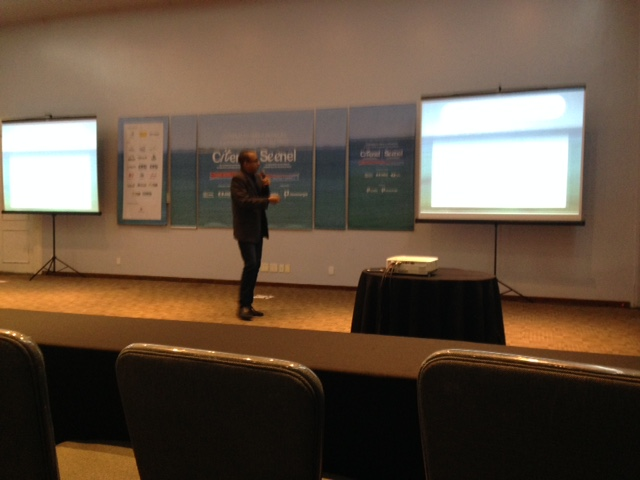
\includegraphics[width=\columnwidth]{figs/inmetro.JPG}
	\caption{Ilustração da palestra Segurança Cibernética em Smart Metering.}
	\label{fig::inmetro}
\end{figure} %Elael
%
\textbf{Produção de Lote Pioneiro de Sensor Inteligente:}

Foram apresentados sensores de voltagem e corrente para linhas de transmissão
que podem tanto ser alimentados pela rede secundária 220V ou por painel solar
(100mW) caso esta não esteja disponível. Cada sensor consome 14mW e se comunica
por GPRS, onde seus dados são exibidos em um software com indicação para cada
local instalado.
A instalação de cada sensor consome entorno de 40min. A análise do impacto do
primeiro lote no tempo de resposta da operadora da rede em caso de avarias na
rede se mostrou muito mais curto, com reduções de até 1h ou 2h,
figura~\ref{fig::bebado}.

\begin{figure}[h!]	
	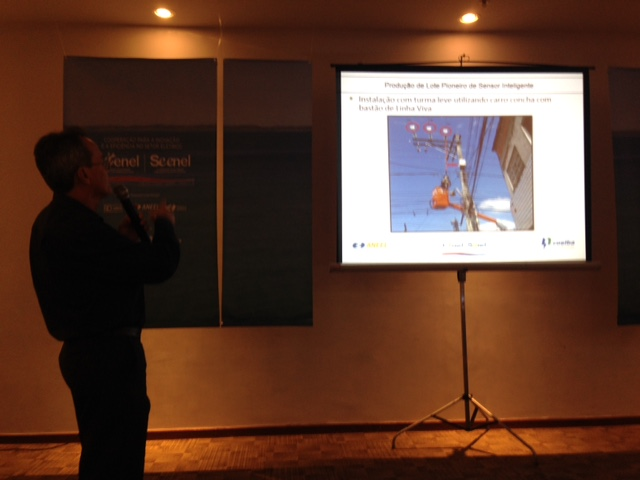
\includegraphics[width=\columnwidth]{figs/bebado.JPG}
	\caption{Ilustração da palestra Produção de Lote Pioneiro de Sensor Inteligente}
	\label{fig::bebado}
\end{figure}
%\input{palestra15} %NOT
%\input{palestra16}
%
\textbf{Instalação de Gerador Solar Fotovoltaico na Aeronáutica Conenectado á
Rede Elétrica do Sistema Isolado de Fernando de Noronha:}


\textbf{Desenvolvimento de sistema robótico para inspeção visual de chaminés e
caldeiras em usina termelétrica:}

Desenvolvimento de um robô escalador de 20 kg com esteiras e rodas para
locomoção e adesão por íma permanente (magnetismo). A aplicação é inspeção de caldeiras,
espaço confinado com obstáculos, temperatura de até $80^o$C, e paredes com tubos
horizontais. As esteiras são protegidas com resina para não danificar a caldeira
e os tubos aletados. O robô possui iluminação, câmeras HD para navegação, e
sensores de infravermelho para medir distâncias. O robô é operado remotamente
por WiFi e sua energia é fornecida através de umbilical. O grande desafio
técnico foi o desenvolvimento das esteiras e acoplamento dos ímãs. A continuação
do projeto prevê a utilização de sistemas de ultrassom.
 %Renan

\textbf{Sistema de aeronaves não tripuladas multiplataforma de longo alcance
para inspeção de linhas de transmissão:}

Realizado por um grupo do ITA, este trabalho gerou 15 dissertações de
mestrado, 10 teses de doutorado e 15 trabalhos de conclusão de curso, 12 artigos internacionais e 12
artigos nacionais. O projeto consiste em dois veículos aéreos não tripulados
(VANTs) com autonomia de 3h a 4h, 25 kg a 50 kg de massa, e 7 kg a 14 kg de
carga (\textit{payload}). O VANT é catapultado e um piloto é responsável por
guiá-lo remotamente. O VANT sobrevoa próximo à linha de transmissão de energia
elétrica para inspeção. Foi realizado estudo de interferência eletromagnética da linha nos
diversos sensores que compõe o VANT e é feita uma análise de zona ótima para o
vôo, considerando a zona de exclusão devido à interferência e possibilidade de
colisão, e distância mínima necessária para inspeção por câmeras. A tecnologia
por hélices (Drones) mostraram resultados ruins devido à autonomia de apenas 15
minutos. A comunicação entre o VANT e o piloto foi amplificada por um balão, e
esse sistema de retransmissão foi um grande avanço técnico com pedido de
patente.
 %Renan

\textbf{Concepção de um sistema para organização e processamento de imagens
multiespectrais, multitemporais e georeferenciadas de reservatórios para
monitoramento de bordas:}

Sistema de comparação de imagens amostradas em diferentes épocas, meses ou anos,
para monitoramento de reservatórios. O sistema é capaz de classificar pixels da
imagem em estruturas, construções, e outras formas. As imagens são adquiridas
via satélite, o que exige certo investimento, e o custo pode chegar a
R\$100.000,00 para duas a três coletas de imagem de média resolução por ano,
sendo que o comum é realizar aquisição a cda 2 meses, logo o monitoramento não é
em tempo real. O armazenamento das imagens é realizado em PotgreSQL e a
implementação do sistema é feita em PyQGIS (python). O desafio técnico consiste,
principlamente, na correção de angulação da imagem de satélite, a projeção
linear, e a manipulação de matrizes (imagem) para a diferenciação e
classificação.
 %Renan


\section{Conclusões}


%---------------------------------------------------------------------
\end{document}
